\section{M}

    \subsection*{Metrica}

        Una metrica è un indicatore utile a misurare andamenti di interesse.
        Viene utilizzata per controllare, ad esempio, costi di produzione, qualità del prodotto.
        Esistono metriche standard ma possono anche essere create ad-hoc in base ai parametri che si 
        vogliono misurare.

	\subsection*{Milestone}
	
		Le milestone vengono spesso fissate nella fase di pianificazione e sono punti sull'asse temporale che indicano traguardi intermedi significativi nello svolgimento di un progetto; il mancato raggiungimento di una milestone indica che il progetto non sta procedendo come pianificato e devono essere applicate delle misure correttive.

	\subsection*{Modello a V}
		Identifica come strategia di verifica e validazione del prodotto la sequenza: test delle unità, test di integrazione, test di sistema, test di accettazione. Il superamento di ognuno di questi passi conferma il successo nell'implementazione del corrispettivo prodotto intermedio del processo di sviluppo fino a validare il software rispetto al contenuto del Capitolato, come da figura.
		\\
		\begin{figure}[H]
                \centering
                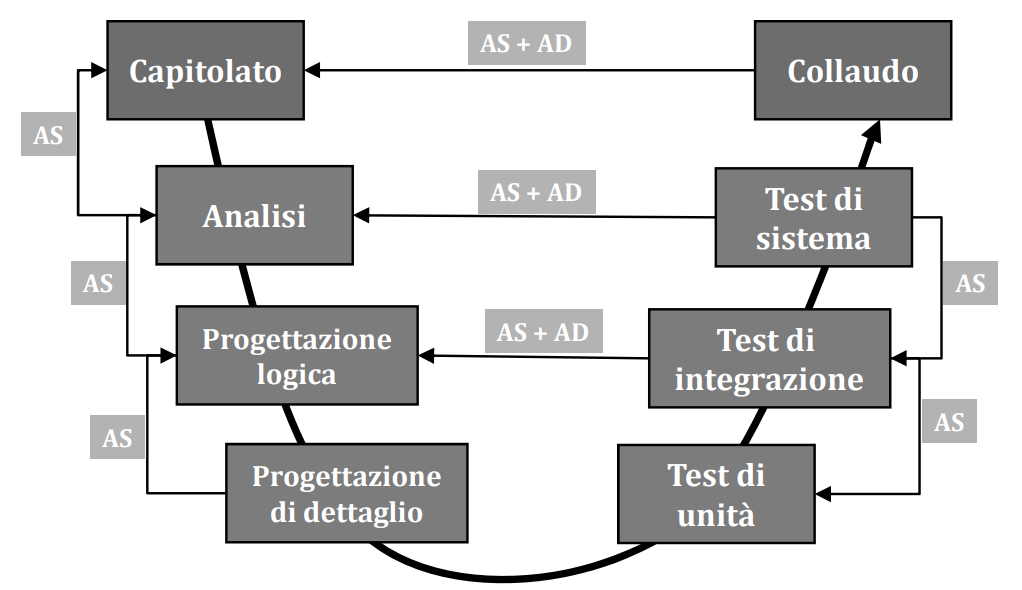
\includegraphics[width=14cm,height=14cm,keepaspectratio]{./images/modello_v.png}
                \caption{rappresentazione Modello a V}
        \end{figure}

    \subsection*{Modello incrementale}

        In ingegneria del software, il modello incrementale è un modello di sviluppo software basato sulla successione di
        una serie di passi. Il ciclo dei passi può essere iterativo fino al soddisfacimento dei requisiti del cliente.
        Questo modello ha il vantaggio di creare prototipi che favoriscono l'interazione con il cliente così da favorire
        il dialogo e la validazione dei requisiti.
